\subsection{Kandidatensuche}\label{sec:kandidatensuche}
Die Kandidatensuche, im Folgenden Suche genannt, wird über eine klassische Graphensuche durchgeführt, wobei der vollständige
Graph alle möglichen Stösse enthält.
Für die Suche gibt es zwei Möglichkeiten, entweder wird bei der weissen Kugel gestartet und von dort ein Stoss gesucht,
welcher eine andere Kugel ins Loch spielt, oder es wird bei einem oder mehreren Löchern gestartet und von dort ein Stoss gesucht,
welcher von der weissen Kugel ausgehend eine andere Kugel ins Loch spielt.

Nachfolgend wird die Suche beschrieben, welche beim Loch, dem Ziel, startet, eine einzulochende Kugel findet
und anschliessend den Stoss bis zur weissen Kugel zurück sucht.
Dementsprechend ist der Root-Knoten des Suchbaumes das zu treffende Ziel (Loch).
Da ein handelsüblicher Billiardtisch mehrere Löcher hat, muss pro Loch eine separate Suche durchgeführt werden.

Bei der Durchführung eines Expansionsschrittes werden ausgehend von einem Knoten im Suchbaum dessen Nachfolger-Knoten ermittelt.
Diese stellen im Fall vom Root-Knoten Kugeln dar, welche in dieses Loch gespielt werden könnten.
Aus diesen Kugeln werden Kugel-Knoten gebildet, welche diese Kugeln entweder auf direktem Wege oder indirekt über die Bande
in das Loch spielen lassen sollen.
Ausgehend von diesen Kugel-Knoten, werden deren Nachfolger-Knoten in weiteren Expansionsschritten ermittelt, welche
wiederum Kugel-Knoten darstellen.
Diese Kugel-Knoten stellen dann Kugeln dar, welche die Kugel des Vorgänger-Kugel-Knotens entweder auf direktem Wege oder indirekt
über die Bande treffen sollen.
Sofern ein Kugel-Knoten die weisse Kugel darstellt, so ist dieser Kugel-Knoten ein Endzustand und damit ist der Stoss
über die Kette von Nachfolger- zu Vorgänger-Kugel-Knoten definiert.

Zur Veranschaulichung des Prinzips folgt ein Beispiel.Es wird vereinfacht angenommen,
dass der Tisch nur ein Loch hat. Für mehrere Ziele ergeben sich mehrere Suchbäume, einen pro Loch.
In Abbildung \ref{fig:backwardsearch_1} erfolgt die Eingabe des Suchalgorithmus in Form des Root-Knotens.
Es wird nur das zu treffende Ziel definiert. Auf der rechten Seite des Tisches ist der Suchbaum dargestellt.

\begin{figure}[h!]
    \begin{center}
        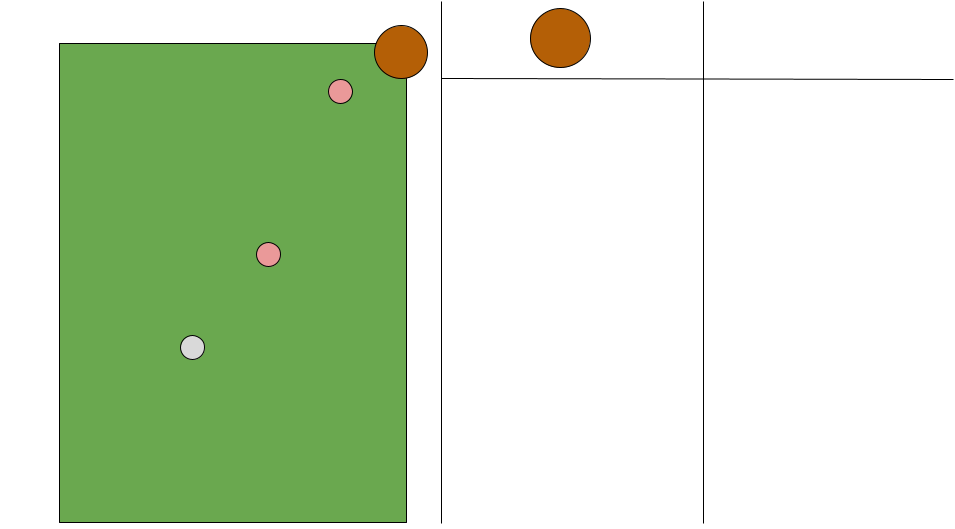
\includegraphics[width=0.5\linewidth]{../common/03_billiard_ai/resources/11_backwardsearch_1.png}
    \end{center}
    \caption{Kandidatensuche 1}
    \label{fig:backwardsearch_1}
\end{figure}

In einem zweiten Schritt wird die einzulochende Kugel definiert. Es kommen lediglich die beiden roten Kugeln in Frage.
Nachfolgend wird der Pfad weiter betrachtet, bei dem die rote Kugel, welche näher beim Loch ist, gewählt wurde.
Abbildung \ref{fig:backwardsearch_2} zeigt, dass der Suchbaum um einen Knoten erweitert wurde.
\begin{figure}[h!]
    \begin{center}
        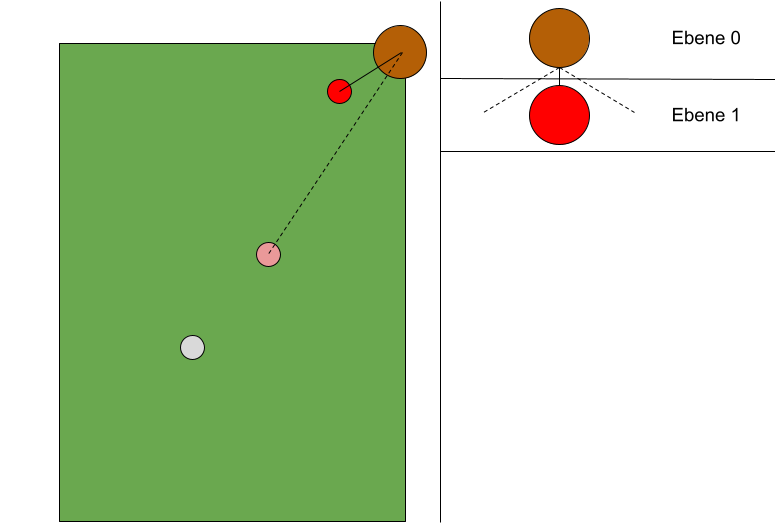
\includegraphics[width=0.5\linewidth]{../common/03_billiard_ai/resources/12_backwardsearch_2.png}
    \end{center}
    \caption{Kandidatensuche 2}
    \label{fig:backwardsearch_2}
\end{figure}

In Abbildung \ref{fig:backwardsearch_3} erfolgt der letzte Schritt. Hier sind verschiedene Optionen möglich, bspw.
könnte die weisse Kugel direkt oder über die Bande an die zuvor gewählte rote Kugel gespielt werden. Es könnte aber auch
die andere rote Kugel an die zuvor gewählte rote Kugel gespielt werden. Hier wird der Fall betrachtet, dass die weisse Kugel
indirekt über eine Bande an die zuvor gewählte rote Kugel gespielt wird.
\begin{figure}[h!]
    \begin{center}
        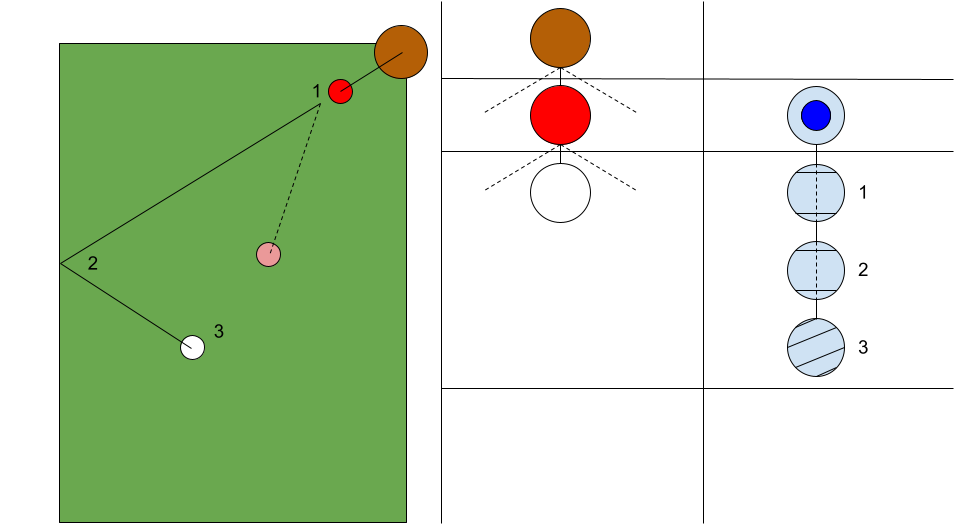
\includegraphics[width=0.5\linewidth]{../common/03_billiard_ai/resources/13_backwardsearch_3.png}
    \end{center}
    \caption{Kandidatensuche 3}
    \label{fig:backwardsearch_3}
\end{figure}

Algorithmus \ref{alg:backward_search} verdeutlicht den ablauf der \glqq Expand-Funktion\grqq. Zuerst wird eine
leere Liste namens \glqq nodes\grqq{} angelegt. Diese wird danach mit Nodes gefüllt, welche entweder durch einen Stoss
über eine weitere Kugel oder indirekt über die Bande zustande kommen. Die Nodes bilden das Ergebnis der Funktion.

\begin{algorithm}[H]
    \DontPrintSemicolon
    \SetKwFunction{expand}{expand}
    \SetKwProg{Fn}{Function}{}{}
    \Fn{\expand{node: Node, constantObjects: list} $\longrightarrow$ list[Node]}{
        nodes $\longleftarrow$ list()\\
        nodes $\longleftarrow$ append(expandBalls(node, constantObjects), nodes)\\
        nodes $\longleftarrow$ append(expandBank(node, constantObjects), nodes)\\
        \KwRet nodes
    }
    \caption{Algorithmus zur Durchführung eines Expansionsschritts bei der Kandidatensuche}
    \label{alg:backward_search}
\end{algorithm}

\subsubsection{Bewertungsfunktion}
Um die Suche zu vereinfachen und in eine spezfische Richtung zu lenken, wo die besten Resultate zu erwarten sind, ist
es unerlässlich eine Bewertung des Stosses durchzuführen. Die Heuristik wurde so definiert, dass sie sich auf den
aktuell expandierten Knoten beschränkt. Die Kosten für eine Expansion werden über die Pfade aufsummiert. Anhand der
Summen kann jeweils der kostengünstigste Pfad evaluiert und verfolgt werden.
Das Prinzip wird in Abbildung \ref{fig:suchbaum_bewertung} veranschaulicht. Die Knoten werden je nach Bedeutung mit
unterschiedlichen Farben markiert. Blau sind sie, wenn sie bereits expandiert wurden. Grün, wenn der Knoten im nächsten
Schritt expandiert wird, da er die geringsten Pfadkosten aufweist und rot, wenn der Knoten nicht in Frage kommt aufgrund
zu hoher Kosten. Dieses Vorgehen entspricht demjenige des Dijkstra-Algorithmus \cite{wiki.dijkstra:1}.
\begin{figure}[h!]
    \begin{center}
        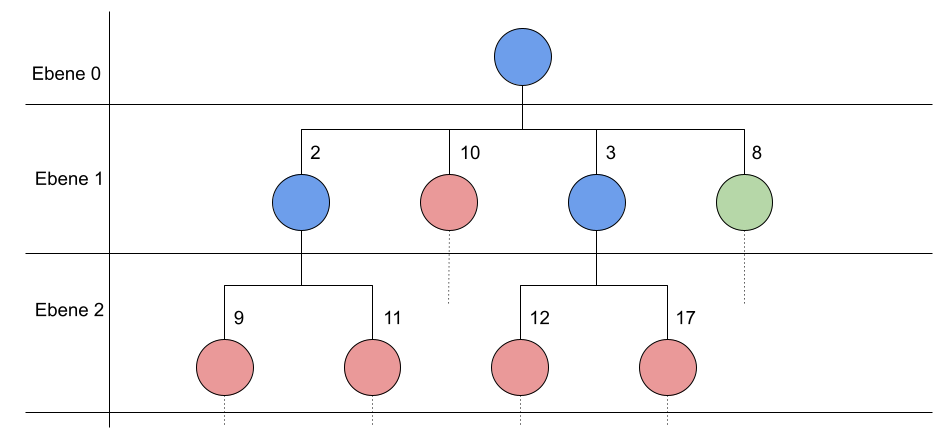
\includegraphics[width=0.8\linewidth]{../common/03_billiard_ai/resources/28_suchbaum_bewertung.png}
    \end{center}
    \caption{Bewertung eines Suchbaums}
    \label{fig:suchbaum_bewertung}
\end{figure}

Die Kosten werden auf Basis dreier Kriterien\footnote{Die Kriterien betreffend der Distanz wie auch des Winkels werden wie
in Publikation \cite{inproceedings:billiard_ai:1} verwendet.} gebildet. Das Erste bildet die Berücksichtigung der Distanz, welche eine
Kugel zurücklegt. Das Zweite behandelt den Winkel, in welcher ein Zielpunkt getroffen werden muss. Das Dritte fügt den
Kosten einen Wert für jede Indirektion hinzu. Jeder dieser Werte liegt zwischen $0$ und $1$.
Die ersten beiden Kriterien sind in Abbildung \ref{fig:suche_knoten_expansionskosten} veranschaulicht.
Es werden zwei Expansionen gezeigt. Die relevanten Informationen $d$ für die Distanz sowie $\alpha$ für den Winkel weisen
einen entsprechenden Index auf, welcher den Expansionsschritt markiert. Beim ersten Expansionsschritt bildet der Zielpunkt
den Elternknoten. Der Winkel $\alpha_1$ ist definiert durch die Rollrichtung der Kugel und einer Normalen auf den Zielpunkt.
Die Normalen zeigen jeweils zum Ursprung in der Mitte des Tisches. Die Distanz $d_1$ ist definiert über die Länge des
zurückzulegenden Weges. Im zweiten Fall wird der Winkel $\alpha_2$ durch die Rollrichtung der ersten und der Rollrichtung
der zweiten Kugel definiert.

\begin{figure}[h!]
    \begin{center}
        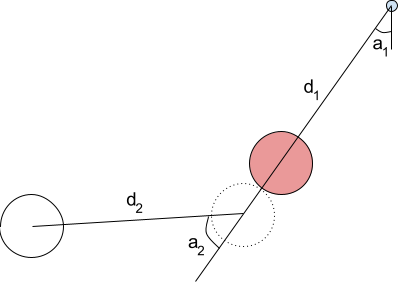
\includegraphics[width=0.5\linewidth]{../common/03_billiard_ai/resources/29_suchbaum_expansionskosten.png}
    \end{center}
    \caption{Expansionskosten eines Knotens}
    \label{fig:suche_knoten_expansionskosten}
\end{figure}

Um die beiden Grössen vergleichen zu können, müssen sie in dieselbe Grössenordnung gebracht werden. Aus diesem Grund
werden sie durch die maximal möglichen Werte normiert\cite{qucosa:ein_billardroboter:1}. Für die Distanz ist dies die
Diagonale über den Tisch, für den Winkel wird ein maximal möglicher Wert von $90^\circ$ gewählt, dies ist bereits bei
der Suche berücksichtigt. Daher kann der Winkel nur noch umgerechnet werden. Die resultierende $0$ beim Cosinus bei $90^\circ$
wird auf $1$ gemappt, die $1$ bei $0^\circ$ auf $1$. Nun gilt die Annahme, dass je kürzer der Weg und je kleiner der Winkel,
desto einfacher der Stoss.
\begin{align}
    d_{krit} = \frac{d_i}{d_{max}}\\
    \alpha^{'}_{krit} = \cos{\alpha} * -1 + 1
\end{align}
Aktuell fliesst der Winkel $\alpha_{krit}$ zu stark in die Bewertung ein. Daher wird dieser durch eine kubische
Bézier-Kurve\cite{wiki.bezier:1} gewichtet. Die Parameter lauten wie folgt.
\begin{align}
    P_0 = \begin{pmatrix} 0 & 0\end{pmatrix}\\
    P_1 = \begin{pmatrix} 1 & 0\end{pmatrix}\\
    P_2 = \begin{pmatrix} 0.5 & 1\end{pmatrix}\\
    P_3 = \begin{pmatrix} 1 & 1\end{pmatrix}\\
    P = \begin{pmatrix} P_0 \\ P_1 \\ P_2 \\ P_3\end{pmatrix}\\
    T = \begin{pmatrix} t^3 & t^2 & t & 1\end{pmatrix}\\
    M = \begin{pmatrix}
            -1 &  3 & -3 & 1\\
             3 & -6 &  3 & 0\\
            -3 &  3 &  0 & 0\\
             1 &  0 &  0 & 0
        \end{pmatrix}\\
    \alpha_{krit} = f(t = \alpha^{'}_{krit})[1] = T \cdot M \cdot P
\end{align}
Nach dieser Gewichtung wird die y-Komponente als $\alpha_{krit}$ verwendet. Die Kurve ist in Abbildung \ref{fig:suche_knoten_gewichtung_winkelkosten}
visualisiert. Es wird deutlich, dass kleinere Winkel einen eher geringen Einfluss auf die Kosten haben.
Ab einem Winkel von $50^\circ$, welche auf der Grafik \ref{fig:suche_knoten_gewichtung_winkelkosten} als Punkt $D_1$ markiert ist,
beginnt die Kurve bis etwa $80^\circ$ stark zu steigen. Ab dort flacht sie wiederum ab, bis die Kosten von $90^\circ$ schliesslich den Wert
$1$ erreichen.

\begin{figure}[h!]
    \begin{center}
        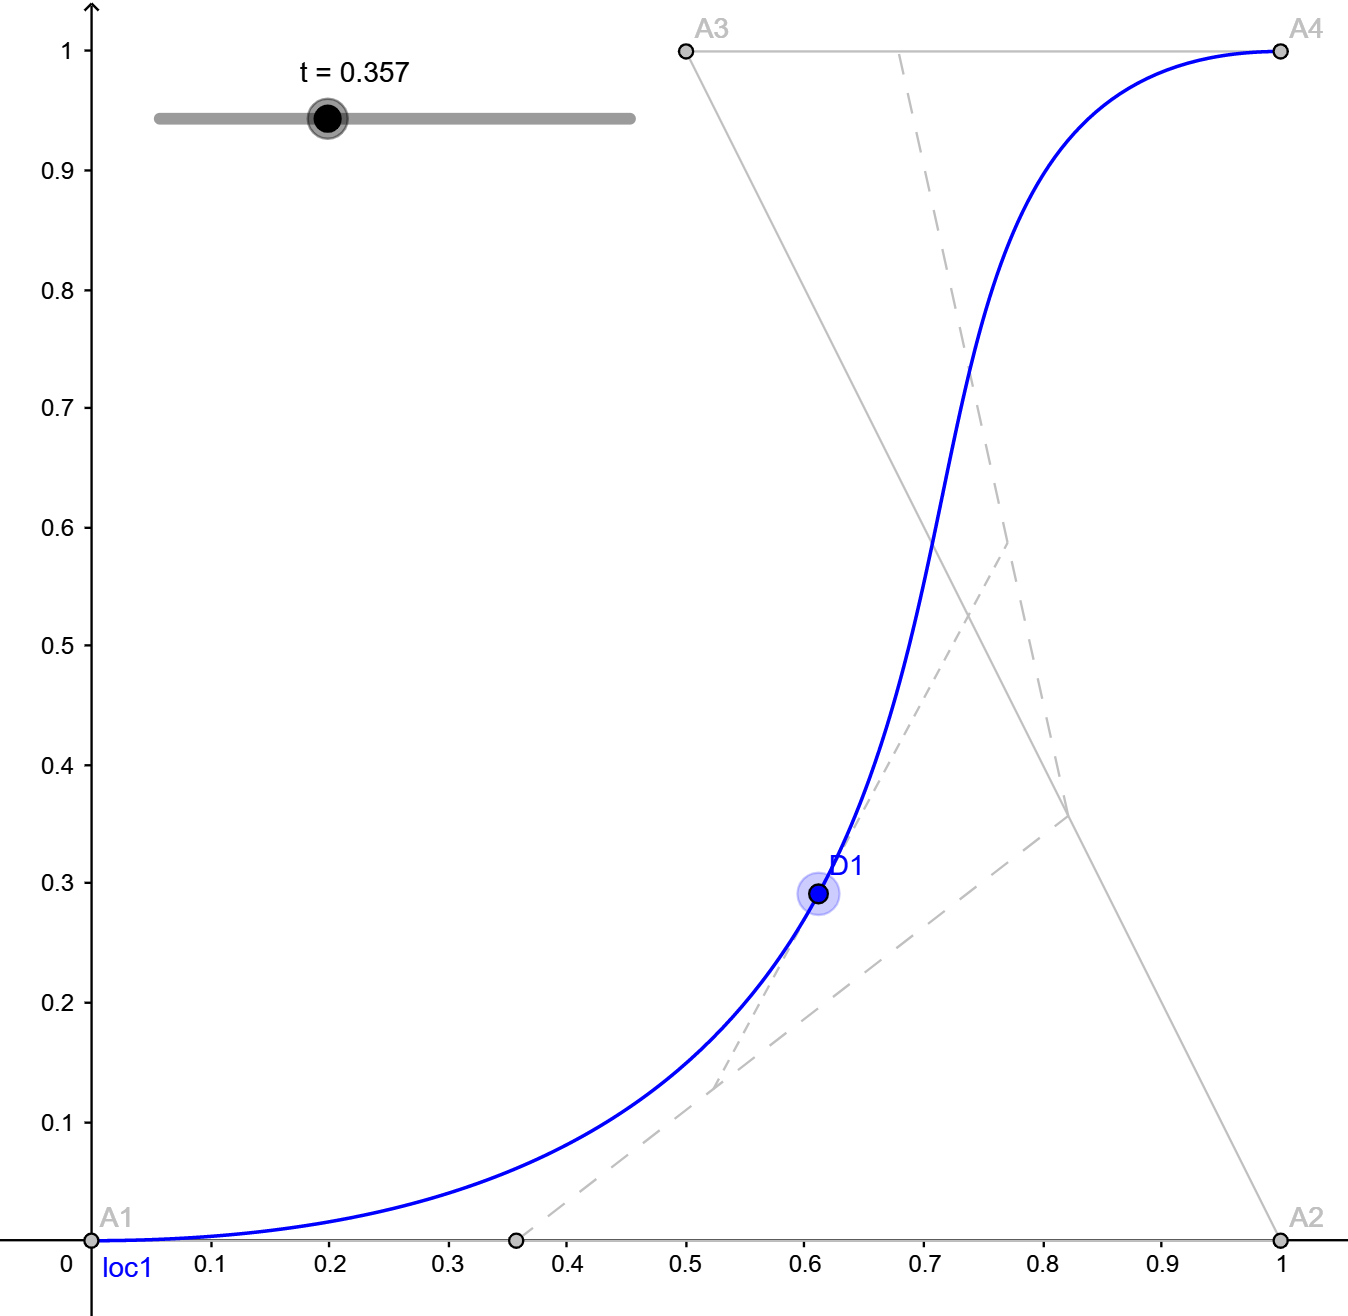
\includegraphics[width=0.6\linewidth]{../common/03_billiard_ai/resources/30_suchbaum_gewichtung_winkelkosten.png}
    \end{center}
    \caption{Gewichtung der Winkelkosten}
    \label{fig:suche_knoten_gewichtung_winkelkosten}
\end{figure}

Das Kriterium der Indirektion über Kugeln wird wiederum über einen maximal möglichen Wert gelöst.
Es wird eine maximale Indirektion $K_{I,max}$ angegeben und die Anzahl der Vorkomnisse ${K_{I,n}}$ wird durch die
Konstante dividiert. Dadurch werden die Kosten erhöht, je grösser der Indirektionsgrad ist.
\begin{align}
    K_{I,krit} = \frac{K_{I,n}}{K_{I,max}}
\end{align}

Die endgültigen Kosten werden über die Addition aller Kriterien gebildet.
\begin{align}
    K = d_{krit} + \alpha_{krit} + K_{I,krit}
\end{align}

TODO: Spezialkosten (Einlochen) erfassen
